\documentclass[11pt]{article}

%\usepackage{tsystyle}
% \usepackage[landscape, margin={3cm,3cm}]{geometry}
% \usepackage{multicol}
% \setlength{\columnsep}{1cm}
%\usepackage{crystaldefs}
% \usepackage[font={small,it}]{caption}
\usepackage{hyperref}
\hypersetup{
    colorlinks=true,
    linkcolor=blue,
    filecolor=magenta,      
    urlcolor=cyan,
    % pdfpagemode=FullScreen,
    }
\usepackage{graphicx}
% \usepackage{ulem}
% \usepackage{setspace}
\usepackage{amssymb}
\usepackage{amsmath}
\usepackage{epstopdf}
\usepackage{xcolor}
%\usepackage{floatflt}
% \usepackage{fancyhdr}
\usepackage{color}
\graphicspath{{../figs/} {../graphics/}}
% \usepackage{lastpage}
% \usepackage{wrapfig}
% \usepackage[compact]{titlesec}
\usepackage[sort&compress]{natbib}

%\DeclareGraphicsRule{.tif}{png}{.png}{`convert #1 `dirname #1`/`basename #1 .tif`.png}
\bibliographystyle{unsrt}

        % \setlength{\oddsidemargin}{-0.3in}
	% \setlength{\evensidemargin}{0.1in}
	% \setlength{\textwidth}{6.4in}
	% \setlength{\topmargin}{-0.5in}
	% \setlength{\textheight}{9.1in}
% \parskip = 0.1in
% \parindent = 0.0in



% \pagestyle{fancy}
% \lhead{}

\def \qdot{\dot{\mathbf{q}}}
\def \qddot{\ddot{\mathbf{q}}}
\def \q{\mathbf{q}}
\def \xp{\mathbf{x}_p}
\def \qdot{\dot{\mathbf{q}}}
\def \xpdot{\dot{\mathbf{x}}_p}
\def \xpddot{\ddot{\mathbf{x}}_p}
\def \qddot{\ddot{\mathbf{q}}}
\def\bs#1{\boldsymbol{#1}}
\def \q{\mathbf{q}}
\def\rmd{{\rm d}}

\newcommand\etc{\textsl{etc}}
\newcommand\eg{\textsl{eg.}\ }
\newcommand\etal{\textsl{et al.}}
\newcommand\Quote[1]{\lq\textsl{#1}\rq}
\newcommand\fr[2]{{\textstyle\frac{#1}{#2}}}
\newcommand\miktex{\textsl{MikTeX}}
\newcommand\comp{\textsl{The Companion}}
\newcommand\nss{\textsl{Not so Short}}

\renewcommand{\th}{\textsuperscript{th}} % ex: I won 4\th place
\newcommand{\nd}{\textsuperscript{nd}}
\newcommand{\st}{\textsuperscript{st}}
\newcommand{\rd}{\textsuperscript{rd}}

\newcommand{\sscr}[1]{\textsuperscript{#1}\,}
\newcommand{\Molacek}{ Mol\'{a}\v{c}ek }
% \renewcommand{\thesection}{\Roman{section}} 
% \renewcommand{\thesubsection}{\thesection.\Alph{subsection}}
\makeatletter

\newcommand{\comment}[1]{\textcolor{red}{#1}}

\begin{document}


\pagestyle{plain}
\author{...}
\title{SIWA: Overlay V3
}
 \maketitle
 \abstract{}
 \begin{center}
	 
\includegraphics[width=2in]{marvel.png}
 \end{center}
 \section{Oracle Problem}

% Each endpoint will require its own bespoke solution . In other words, reliable on-chain data for some industry  will depend on in-depth knowledge of that industry, and thus will be effected by professionals in that area. Each migration of reliable data onchain 

%  The solution is not to insure endpoints. This is probably impossible. Instead, one should recognize which way the wind is blowing and realize the good news: everything worth caring about will be on the blockchain sooner or later. We can therefore focus on {\it on-chain oracles}. 




 \section{SIWA}
 Let us simplify matters and consider a pure derivatives market, assuming that whenever an investor executes a long or short position they do so out of {\it belief in mispricing} --- i.e. that the price will increase or decrease respectively. The size of the position is proportional to the magnitude of both the  belief and  mispricing. %price change.  

 Then, each trade becomes then an implicit {\it statement} about the future price. Let the time difference between now and the future be $\Delta t$.
% The future time $t$ is the time now $t_0$ plus some time delta $\Delta t$.  
 Uncertainty increases with $\Delta t$. If $\Delta t$ is zero, uncertainty is essentially zero. 
 As both risk and reward grow with uncertainty, %. % which is why options have time decay. 
price oracles can  be considered as trades with zero uncertainty, and thus zero risk and reward. 

A trade with no risk and reward seems like not a trade anymore, which is why thinking about oracles as utilities rather than risk-taking ventures is typically more useful. The conceptual connection between traders and oracles is nevertheless present, and it is this connection that we leverage in SIWA. 

We assume that the users of Overlay are all traders. Traders, however, have different risk profiles. One of the primary insights to come out of Overlay V1 is that these different profiles can be fit together to serve each other and stabilize the system. There are currently two such profiles referenced in protocol design docs: {\it speculators} (i.e. traders or users) and {\it basis} traders (also called carry  traders). In SIWA we  add {\it  creditors}, i.e. those with a large amount of capital who loan it out for interest at very low risk. These are like bond purchasers. 


\begin{center}
\begin{tabular}{|l|c|c|}
	\hline
Speculators & & \\
Basis/carry traders & & \\
Creditors & & \\
\hline
\end{tabular}
\end{center}


 The nature of markets is such that making a statement about future price reduces to making a statement about the statements of others about future price. This is the \href{https://en.wikipedia.org/wiki/Keynesian_beauty_contest}{Keynesian beauty contest}. When $\Delta t = 0$, the choices of others are in theory trivial to predict by simply making an observation, which is the basis of the Schelling coin idea.

 % \begin{enumerate}
	 % \item Floating price
% \item  Basis trade to reduce risk. 
% \item Making an observation
% \end{enumerate}


 \section{Schelling Coin}

 We use a proof of stake system, in which capital (ETH, OVL, DAI etc) is locked by oracles. Either the required amount is fixed to obtain one vote (e.g 32 ETH) or  the weight of each vote is proportional to the locked capital. 

 We identify four separate classes of oracles. 
 \begin{enumerate}
	 \item {\it Trusted}: nodes which are doxxed -- KYC/AML applies  and they may even have a legal agreement with the Overlay Foundation.  
	 \item {\it Sponsor}: nodes which lock an extra amount of OVL as insurance to initially sponsor a feed. They receive outsized rewards but their stake is used to pay back the protocol in case the market they are sponsoring is not suitable (i.e. is predictable or manipulable).
	 \item {\it Honest}: nodes which stake and serve prices faithfully. 
	 \item {\it Attacker}: nodes which stake and attempt to manipulate prices.  
 \end{enumerate}
 Let $T, S, H, A$ be the sets of trusted, sposor, honest, and attacking nodes, respectively. For some individual member $T_i \in T$ we write the amount of capital staked by that individual as $f(T_i)$. Then set 
 \[\hat{T} = \sum_{i=1}^{|T|} f(T_i)\]
 for the total amount of capital staked by all trusted nodes. 

 The main problem with schelling coin is bootstrapping the network to the point that there are enough individual nodes that cheating is almost impossible. We propose a solution to this problem below. The basic idea is to move from pure centralization to pure decentralization in  precisely-defined stages, while handling the attacks specific to each stage.



 \begin{center}
	 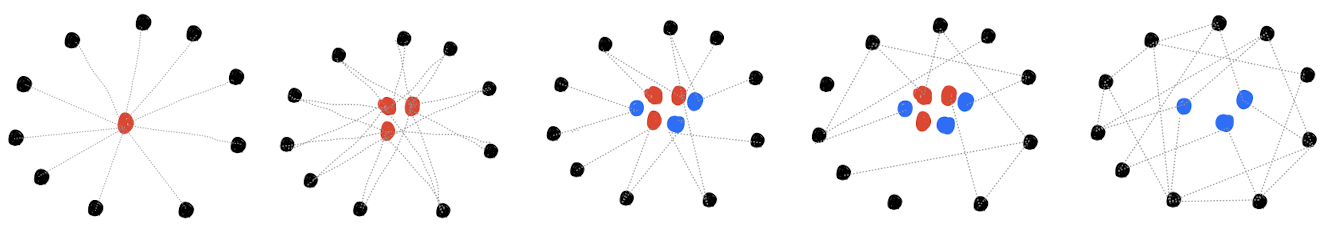
\includegraphics[width=4in]{progression.png}
 \end{center}

 \begin{enumerate}
	 \item Case 1: All sponsors are actually attackers and there are no honest nodes.  

		 In this case, there is no way of reliably serving prices and such a breakdown points to a deeper problem in the market. If sponsors are attackers, then clearly the market is broken. The same is true simply if sponsors and trusted oracles are disagreeing on the price. In this case, the solution is simple: {\it the market is automatically shut down}.

	 \item Case 2: There are trusted and sponsor nodes but attackers and no honest nodes. 

		 The solution here is to set the cap of the underlying market to either  $\alpha(\hat{T} + \hat{S})$ or $\alpha(\hat{T} + \hat{S} + \hat{A})$ where $0 < \alpha < 1$ (leverage and a specific risk analysis are the main determinant of $\alpha$).  There are two ways that $A$ nodes can move the price. 

		 \begin{enumerate} \item If $\hat{A} > \hat{T} + \hat{S}$ then this amounts to a 51\% attack and the price can be set to an arbitrary value. To mitigate this risk we should continue to use TWAPs even in SIWA, and probably even cap maximum price moves in a specific period. This is equivalent to a market going limit up or down. If a market goes limit up more than $n$ times in a given period (maybe $n=2$), {\it the market is automatically shut down}.

			 This limits damages to ~ $\ell C nb$, where $\ell$ is leverage, $C$ is the cap, and $b$ is the percentage change  in price before the market is limit up. (We could just copy the CME here, but on a much smaller per-TWAP period.)  

			 After the market is shut down, however, the protocol still has the $\hat{A}$ from attackers in the stake. This can be taken from them, so we must simply set parameters such that 
			 \begin{equation}
				 \hat{A} > \ell C nb.
			 \end{equation}
		 \item More plausible is a microcheating scenario where attackers gradually shift the price in their favor by delivering {\it almost} accurate prices. If $p$ is the fair price and $p^{\dagger}$ is the manipulated price, then each TWAP period, attackers can siphon a total of  

			 \begin{equation}
				 \ell C \Big(\frac{p^\dagger}{p} -1 \Big) 
			 \end{equation}
			in OVL from the protocol. 


			The solution here is the same as before. If we have  $n$  periods during which microcheating is possible, {\it the market is automatically shut down}. So long as we have 

			 \begin{equation}
				 \hat{A} > \ell C n \Big(\frac{p^\dagger}{p} -1 \Big) 
			 \end{equation}
			 then damages can be recovered. 
		 \end{enumerate}

		 We note that the solution to both of these cases requires two important features to hold: 1) a high degree of agreement in  prices between trusted and sponsor oracles, which likely requires prices being taken from centralized locations; and 2) a governing body that can review  suspicious events after they occur. (Ideally this is an external paid auditing firm.) 
\subitem 



	 \item Case 3:
	 \item Case 4:
 \end{enumerate}






 % The connection between information and price is analytic (discoverable by reflection). 

% This is the standard idea of information being expressed by price, of events being `priced in', 

 \section{Almost Arbitrary Blockchain Oracles}


 \end{document}
